% !TEX TS-program = pdflatex
% !TEX encoding = UTF-8 Unicode

% This file is a template using the "beamer" package to create slides for a talk or presentation
% - Talk at a conference/colloquium.
% - Talk length is about 20min.
% - Style is ornate.

\documentclass{beamer}

\mode<presentation>
{
  \usetheme{Marburg}
  \setbeamercovered{transparent}
  % or whatever (possibly just delete it)
}


\usepackage[english]{babel}
\usepackage[utf8]{inputenc}
\usepackage{colortbl}

\usepackage{proof} % proof.sty voor derivaties


\usepackage{tikz}
\tikzset{
    embedding/.style={rectangle,draw=black,text centered},
    index/.style={circle,draw=black,text centered, text width=0.45cm},
    hidden/.style={rectangle split,rectangle split horizontal=true,rectangle split parts=7,draw=black},
}
\usetikzlibrary{shapes}
\usetikzlibrary{positioning,backgrounds}


%\usepackage{times}
%\usepackage[T1]{fontenc}
% Or whatever. Note that the encoding and the font should match. If T1
% does not look nice, try deleting the line with the fontenc.

\newcommand{\pijl}[0]{$\rightarrow$}
\newcommand{\hatv}[1]{\overset{\wedge}{\mathstrut#1}}
\renewcommand{\vec}[1]{\mathbf{#1}}

\newcommand{\shaded}{\cellcolor{blue}} 
\newcommand{\focus}{\cellcolor{red}}


%figures:
%\usepackage{tikz}
%\usetikzlibrary{trees,positioning,backgrounds}
%\usetikzlibrary{shapes.multipart}
%\usepackage{tikz-qtree}

\usepackage{algorithm2e}
\usepackage{algorithmic}
\usepackage{float}
\usepackage{graphicx}

\newenvironment{dia}
{
\begin{frame}[fragile, environment=dia]
\frametitle{\insertsection
\ifx\insertsubsection\empty\else
      \,~-~\insertsubsection             % insert current section [should only be done if section defined] 
   \fi}
}
{
\end{frame}
}


\title{Multilingual Distributional Semantics}
\author[Kruit \and Veldhoen]{Benno Kruit \and Sara Veldhoen}
\date{January 13, 2015}



% Delete this, if you do not want the table of contents to pop up at
% the beginning of each subsection:
%\AtBeginSection[]
%{
%  \begin{frame}<beamer>{Outline}
%    \tableofcontents[currentsection]
%  \end{frame}
%}


% If you wish to uncover everything in a step-wise fashion, uncomment the following command: 
%\beamerdefaultoverlayspecification{<+->}


\begin{document}

\begin{frame}
  \titlepage
\end{frame}

\begin{frame}{Outline}
  \tableofcontents   %[pausesections]
\end{frame}

\section{Introduction - related work}
\section{Our first idea (and why it wouldn't work)}
\section{Our new idea}

\begin{dia}
\begin{figure}

\center
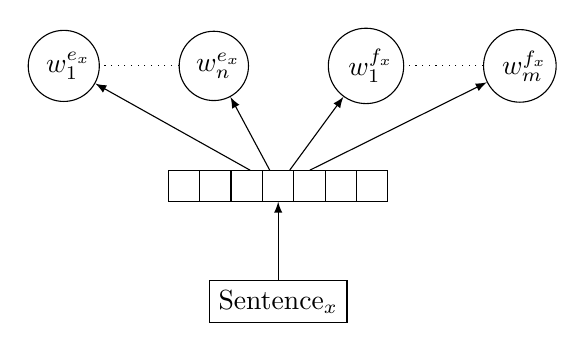
\begin{tikzpicture}[>=latex] 
\node[embedding] (Sx) {Sentence$_x$};
\node[hidden] (h1)[above=of Sx]{} edge [<-] (Sx);
\node[index] (We1) [above left =of h1] {$w^{e_x}_1$} edge [<-] (h1);
\node[index] (Wen) [right =of We1] {$w^{e_x}_n$}edge [<-] (h1) edge [ dotted ] (We1);
\node[index] (Wf1) [right =of Wen] {$w^{f_x}_1$}edge [<-] (h1) ;
\node[index] (Wfm) [right =of Wf1] {$w^{f_x}_m$}edge [<-] (h1) edge [ dotted ] (Wf1);
\end{tikzpicture}
\caption{Bilingual dbow}
\label{f:bilingual_dbow}
\end{figure}
\end{dia}

\begin{dia}
\begin{itemize}
\item Training a single embedding for parallel sentences
\item Word embeddings are not trained
\item Can be extended to more than two languages
\end{itemize}
\end{dia}

\begin{dia}
\begin{itemize}
\item Use sentence embeddings to obtain word vector: 
\begin{equation*}
w=\frac{1}{freq(w,D)}\sum_{s\in D}\sum_{w'\in s} s
\end{equation*}
\end{itemize}
\end{dia}


\section{Evaluation and results}
\section{Graphics and concluding words}




\end{document}
